%!TEX program = xelatex
\documentclass[11pt]{beamer}

\usepackage{amsfonts}
\usepackage{amsmath}
\usepackage{blindtext}
\usepackage{enumitem}

\usetheme{SaoPaulo}

\title{Python Basics!}
\subtitle{mutability, container methods}
\author{CS101 Lecture \#9}
\date{2016-09-21}

\setcounter{showSlideNumbers}{1}

\begin{document}
  \setcounter{showProgressBar}{0}
  \setcounter{showSlideNumbers}{0}

%%%%%%%%%%%%%%%%%%%%%%%%%%%%%%%%%%%%%%%%%%%%%%%%%%%%%%%%%%%%%%%%%%%%%%%%%%%%%%%%
\frame{\titlepage}

%%%%%%%%%%%%%%%%%%%%%%%%%%%%%%%%%%%%%%%%%%%%%%%%%%%%%%%%%%%%%%%%%%%%%%%%%%%%%%%%
\setcounter{framenumber}{0}
\setcounter{showProgressBar}{1}
\setcounter{showSlideNumbers}{1}

%%%%%%%%%%%%%%%%%%%%%%%%%%%%%%%%%%%%%%%%%%%%%%%%%%%%%%%%%%%%%%%%%%%%%%%%%%%%%%%%
\section{Administrivia}

%%%%%%%%%%%%%%%%%%%%%%%%%%%%%%%%%%%%%%%%%%%%%%%%%%%%%%%%%%%%%%%%%%%%%%%%%%%%%%%%
\begin{frame}
  \frametitle{Administrivia}
  \Enlarge
  \begin{itemize}
  \myitem  Homework \#4 is due Friday Sep.\ 23.
  \myitem  Midterm \#1 will be Monday Oct.\ 3.  (evening)
  \end{itemize}
\end{frame}

%%%%%%%%%%%%%%%%%%%%%%%%%%%%%%%%%%%%%%%%%%%%%%%%%%%%%%%%%%%%%%%%%%%%%%%%%%%%%%%%
\section{Warmup Quiz}

%%%%%%%%%%%%%%%%%%%%%%%%%%%%%%%%%%%%%%%%%%%%%%%%%%%%%%%%%%%%%%%%%%%%%%%%%%%%%%%%
\begin{frame}[fragile]
  \frametitle{Question \#1}
  \Enlarge

  \begin{semiverbatim}
a = 1
def fun(a,b):
    return a + b
a = fun( a,a ) + a
  \end{semiverbatim}
  What is the final value of \texttt{a}?
  \begin{enumerate}[label=\Alph*]
  \item  \texttt{2}
  \item  \texttt{3}
  \item  \texttt{4}
  \end{enumerate}
\end{frame}

%%%%%%%%%%%%%%%%%%%%%%%%%%%%%%%%%%%%%%%%%%%%%%%%%%%%%%%%%%%%%%%%%%%%%%%%%%%%%%%%
\begin{frame}[fragile]
  \frametitle{Question \#1 (Worked)}
  \Enlarge

  \begin{semiverbatim}
a = 1
def fun(c,b):
    return c + b
a = fun( a,a ) + a
  \end{semiverbatim}
\end{frame}

%%%%%%%%%%%%%%%%%%%%%%%%%%%%%%%%%%%%%%%%%%%%%%%%%%%%%%%%%%%%%%%%%%%%%%%%%%%%%%%%
\section{Mutability \& Aliasing}

%%%%%%%%%%%%%%%%%%%%%%%%%%%%%%%%%%%%%%%%%%%%%%%%%%%%%%%%%%%%%%%%%%%%%%%%%%%%%%%%
\begin{frame}[fragile]
  \frametitle{Mutability}
  \Enlarge

  \begin{itemize}
  \myitem  We distinguished \emph{mutability} and \emph{immutability}.
  \myitem  The distinction arises from the storage in memory.
  \end{itemize}
  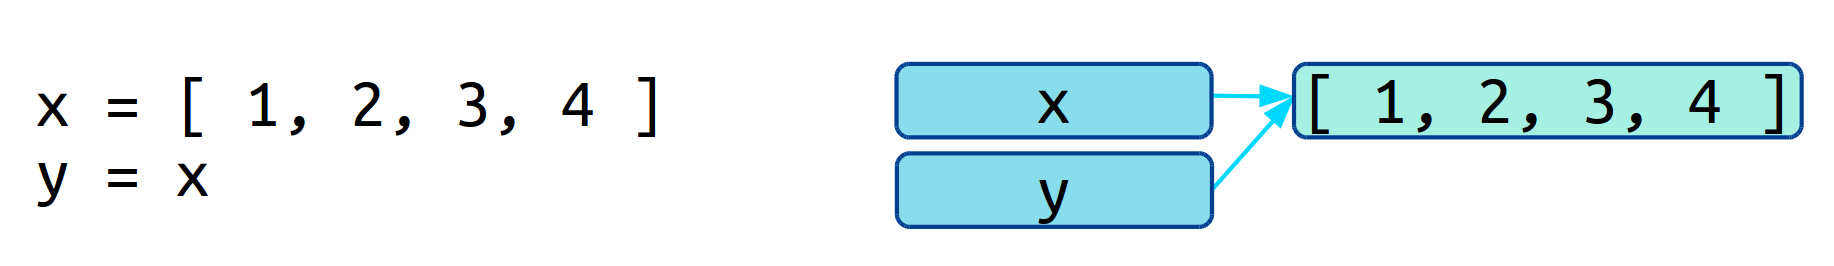
\includegraphics[width=0.8\textwidth]{./img/memory-mutability.png}
\end{frame}

%%%%%%%%%%%%%%%%%%%%%%%%%%%%%%%%%%%%%%%%%%%%%%%%%%%%%%%%%%%%%%%%%%%%%%%%%%%%%%%%
\begin{frame}[fragile]
  \frametitle{Mutability}
  \Enlarge

  \begin{itemize}
  \myitem  \emph{Immutability} occurs when values are copies in memory.
  \end{itemize}
  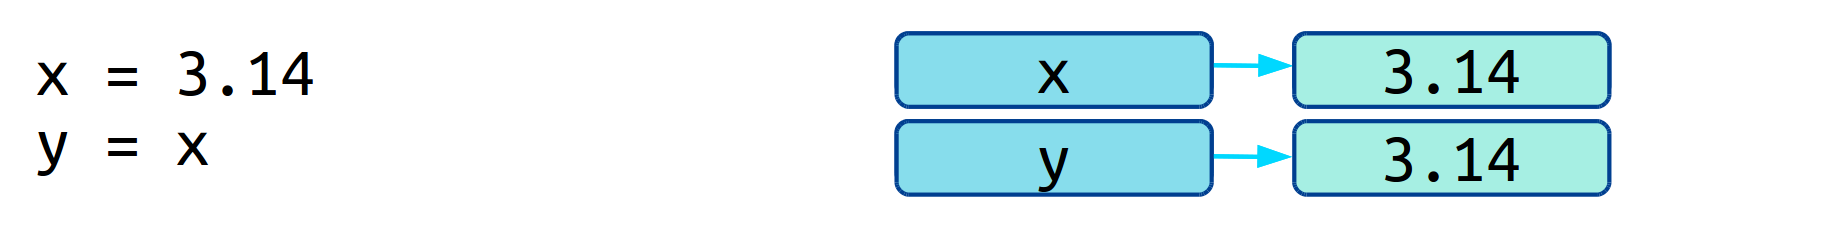
\includegraphics[width=0.8\textwidth]{./img/memory-immutability.png}
\end{frame}

%%%%%%%%%%%%%%%%%%%%%%%%%%%%%%%%%%%%%%%%%%%%%%%%%%%%%%%%%%%%%%%%%%%%%%%%%%%%%%%%
\begin{frame}[fragile]
  \frametitle{Mutability}
  \Enlarge

  \begin{itemize}
  \myitem  \emph{Mutability} occurs when values share the same location.
  \myitem  The distinction arises from the storage in memory.
  \end{itemize}
  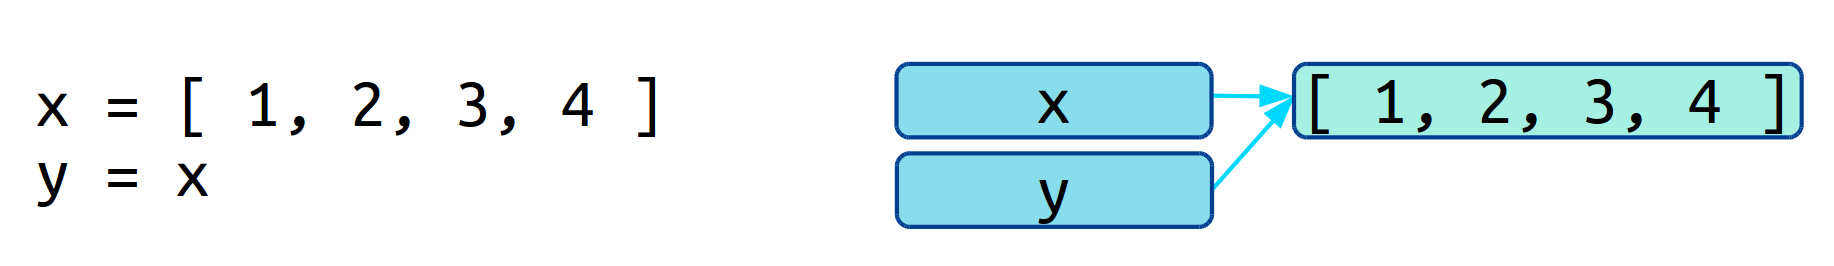
\includegraphics[width=0.8\textwidth]{./img/memory-mutability.png}
\end{frame}

aliasing

  \myitem  The immutable analogue of a \texttt{list} is a \texttt{tuple}.
  \myitem  We form a tuple by using parentheses \texttt{()} instead of square brackets \texttt{[]}.

tuples

indexing
sorting
searching
